\documentclass[a4paper]{ctexart}
\usepackage[top=2.3cm,bottom=2cm,left=1.7cm,right=1.7cm]{geometry} 
\usepackage{amsmath} 
\usepackage{booktabs}
\usepackage{amsthm}
\usepackage{longtable} 
\usepackage{graphicx}
\usepackage{subfigure}
\usepackage{caption}
\usepackage{fontspec}
\usepackage{titlesec}
\usepackage{fancyhdr}
\usepackage{subfig}
\def\degree{$^{\circ}$}
\def\mm{\mathrm{mm}}
\def\cm{\mathrm{cm}}
\def\nm{\mathrm{nm}}
\def\V{\mathrm{V}}
\def\m{\mathrm{m}}
\def\g{\mathrm{g}}
\def\s{\mathrm{s}}
\def\i{\mathrm{i}}
\title{\textbf{光衍射的定量研究}}
\author{王崇斌 1800011716}
\date{}
\makeatletter %使\section中的内容左对齐
\renewcommand{\section}{\@startsection{section}{1}{0mm}
	{-\baselineskip}{0.5\baselineskip}{\bf\leftline}}
\makeatother
\begin{document}
	\pagestyle{fancy}
	\lhead{普通物理实验报告} 
	\chead{}
	\rhead{}
	\maketitle
    \thispagestyle{fancy}
    \section{\large{数据处理}}
    \subsection{单缝衍射}
    \par 
    首先给出单缝衍射时的数据信息,选择单缝III-7;狭缝位置28.00cm,光探测器位置93.90cm,
    同时还要考虑真实的探测器与底座之间的距离4mm,这样可以计算得到狭缝到探测器的距离$d=663\;\mm$。
    我们首先给出单缝衍射实验原始数据所画出的图形,并且使用衍射一级斑光强极大值与零级斑
    光强最大值出现的位置粗略计算出狭缝的宽度。
    \begin{figure}[htbp]
        \centering
        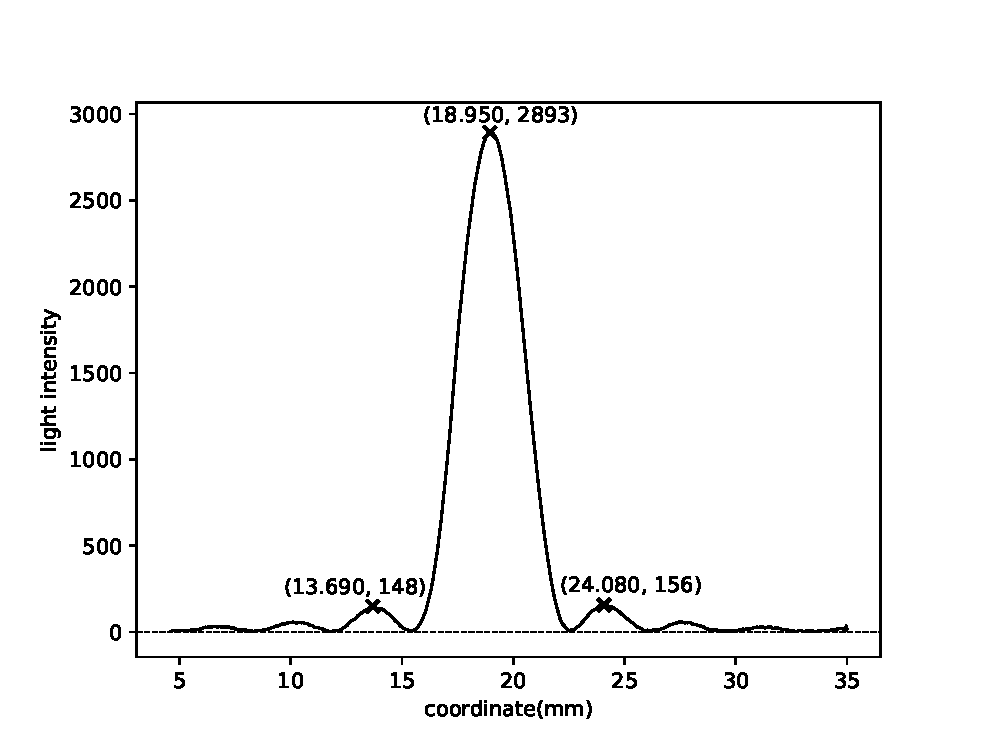
\includegraphics[scale=0.8]{image/single_original.eps}
        \caption{单缝衍射的光强随探测器位置分布的原始数据图}
    \end{figure}
    \par 
    图中标出了测得的零级斑的最大光强$I_{0}$、两个一级斑光强$I_{1},\;I_{2}$以及出现的位置。根据
    单缝衍射的公式:
    \begin{equation}
    I = I_{0} \left(\frac{\sin u}{u}\right)^{2},\;\; u = \pi a\frac{\sin \theta}{\lambda}
    \end{equation}
    公式中$a$为狭缝宽度,$\theta$为衍射图样相对于衍射屏的张角。由上述公式经过求导可得到一级斑的光强
    极大值出现在:
    \begin{align*}
    \sin \theta &= \pm 1.43 \frac{\lambda}{a}\\
    \sin \theta &\approx \frac{24.080 - 13.690}{2 \times 663} = 7.84 \times 10^{-3}\\
    a &= 1.43\frac{\lambda}{\sin \theta} = 1.43 \times \frac{632.8}{7.84}\;\mathrm{\mu m} = 115 \mathrm{\mu m}
    \end{align*}
    \\
    \par 
    下面使用拟合的方式来计算$a$,即将公式(1)中的$a$当作参数,同时考虑到光强的测量由一定
    的不确定性,考虑$I_{0}$也为参数,使用python的scipy.optimize.curve\_fit进行最小二乘
    拟合,得到拟合后的参数:$a = 114.5\mathrm{\mu m},\;\;I_{0} = 2939$
    \begin{figure}[htbp]
        \centering
        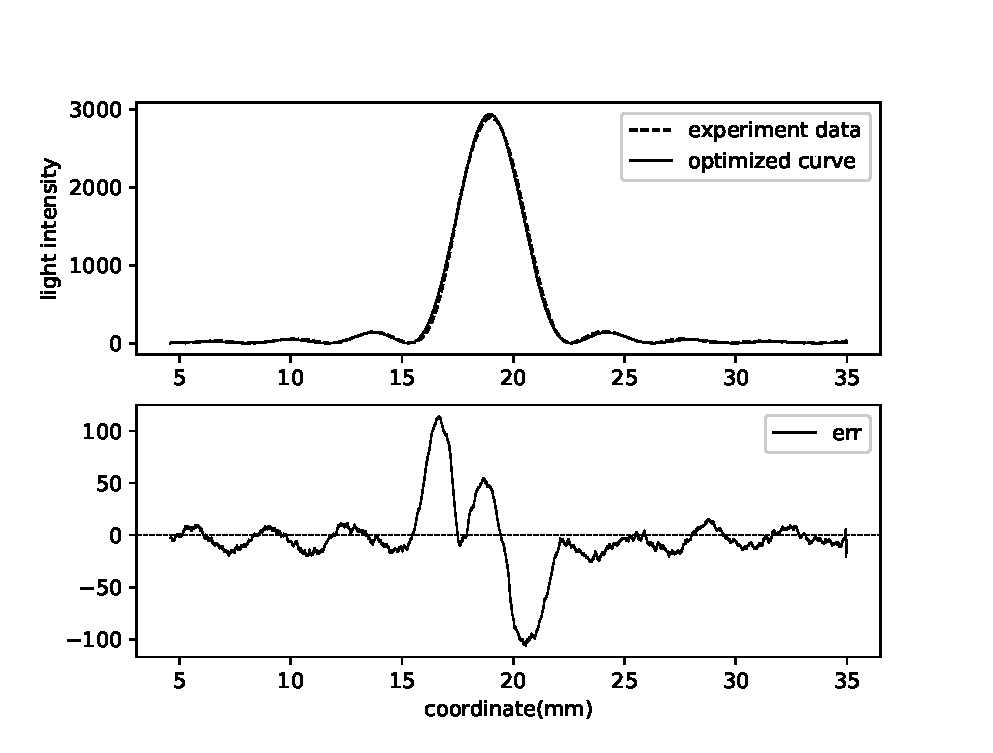
\includegraphics[scale=0.8]{image/single_fit.eps}
        \caption{(1)拟合曲线与实验曲线的对比\;\;(2)残差图}
    \end{figure}
    \par 
    从图上可以看出,在整个测量区域内实验数据与理论相当一致。从残差图上可以进一步看出
    ,在中间光强较大的位置理论与实际出现了较大的偏差,尤其是在中部光强较大的地方。进
    一步观察偏差的特点,发现并不是光强的绝对值较大就会有更大的绝对偏差,最大的偏差出
    现在光强曲线导数绝对值最大的地方,这里给出一个可能的猜测:探测器在测量时光强测量
    与距离测量不是同步的,可能会有微小的时间差,如果光强测量相对于距离测量有一定的
    延迟,那么就会出现实验中那样在光强增大时测量值小于理论值、光强减小时测量值大于理论
    值的情况。
    \subsection{双缝衍射}
    \par 
    首先给出相关数据。探测器底座位置93.90cm,狭缝位置28.50cm,探测器距离底座的距离
    4.0mm。可以得衍射屏与探测器之间的距离为658mm。首先给出实验数据所绘制的衍射光强
    随探测器位置的分布。
    \begin{figure}[htbp]
        \centering
        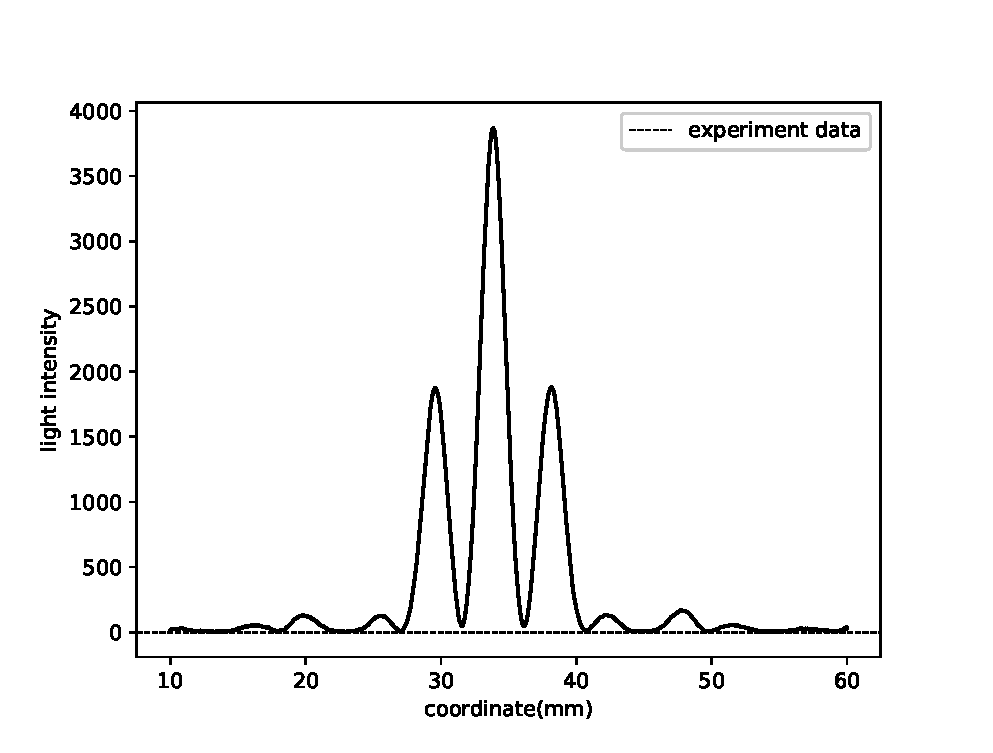
\includegraphics[scale=0.85]{image/double_original.eps}
        \caption{双缝衍射光强随距离分布的原始数据}
    \end{figure}
    \par 
    从图中我们就可以看出双缝衍射与单缝衍射的明显差异,光强分布图中的峰变多了,也变得
    更加细锐,这正是多缝衍射的特点之一。最高峰出现在33.850mm处。
    \par 
    这次我们采用直接拟合的方法来确定相关的参数,首先给出理论公式:
    \begin{equation}
        I = I_{0} \left(\frac{\sin u}{u}\right)^{2} \left(\frac{\sin N \beta}{\sin \beta}\right)^{2},\;\;
        u = \pi a \frac{\sin \theta}{\lambda},\;\; \beta = \pi d \frac{\sin \theta}{\lambda}
    \end{equation}
    \par 
    上式中$N$应取值2,将$I_{0},\; a,\; d$当作参数,使用python的scipy.optimize.curve\_fit进行最小二乘
    拟合(这里必须将光强作为一个参数,因为测出的极强光强并不是$I_{0}$)得到拟合后的参数:
    $a = 41.8 \mathrm{\mu m},\;\; 91.2 \mathrm{\mu m}$。
    \begin{figure}[htbp]
        \centering
        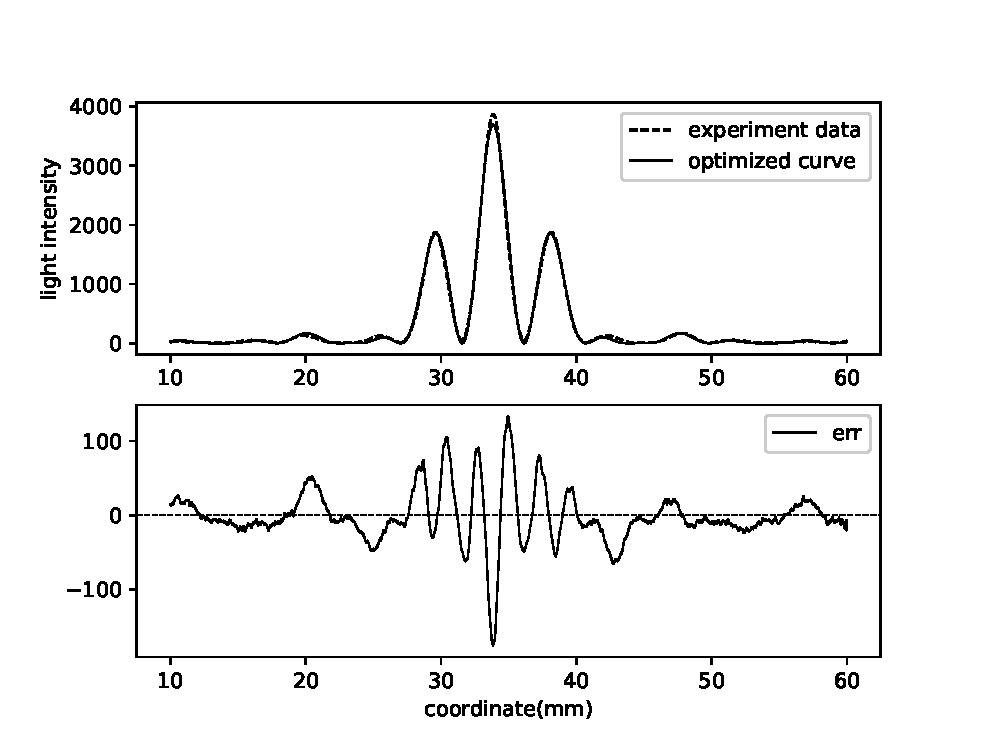
\includegraphics[scale=0.85]{image/double_fit.eps}
        \caption{(1)实验曲线与拟合曲线的对比\;\;(2)残差图}
    \end{figure}
    \par 
    从残差图中可以看出,与理论的偏差依然明显体现在曲线导数较大的地方,除了主极大外,其余峰谷两者相差并不明显。
    \subsection{三缝衍射}
    \begin{figure}[htbp]
        \centering
        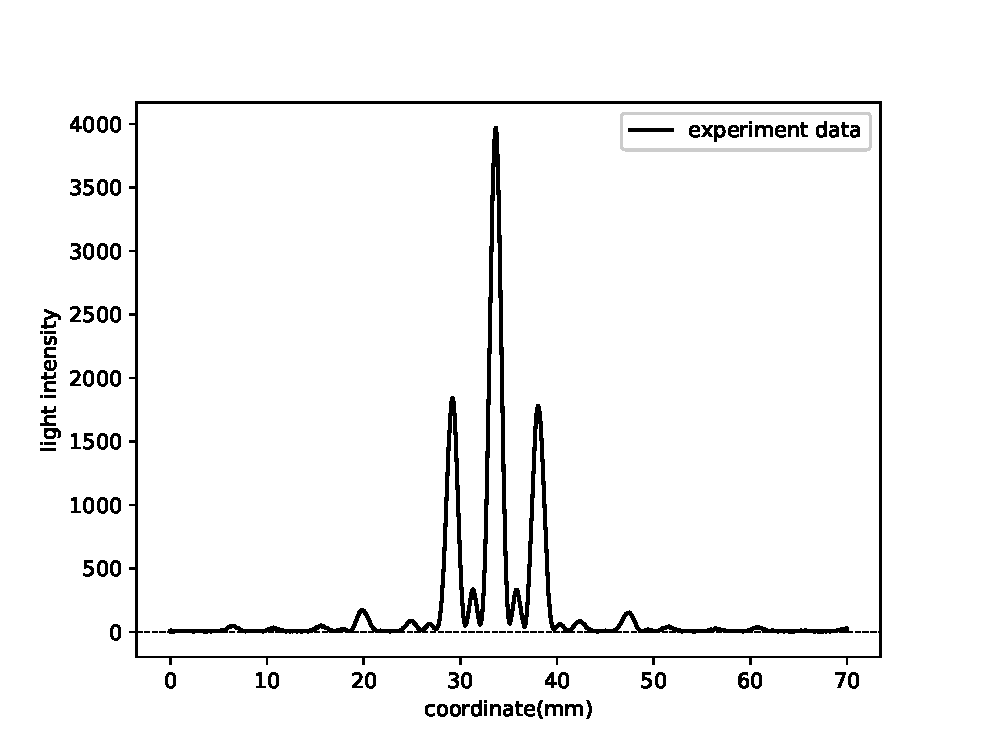
\includegraphics[scale=0.70]{image/triple_original.eps}
        \caption{三缝衍射光强随位置的分布图}
    \end{figure}。
    \begin{figure}[htbp]
        \centering
        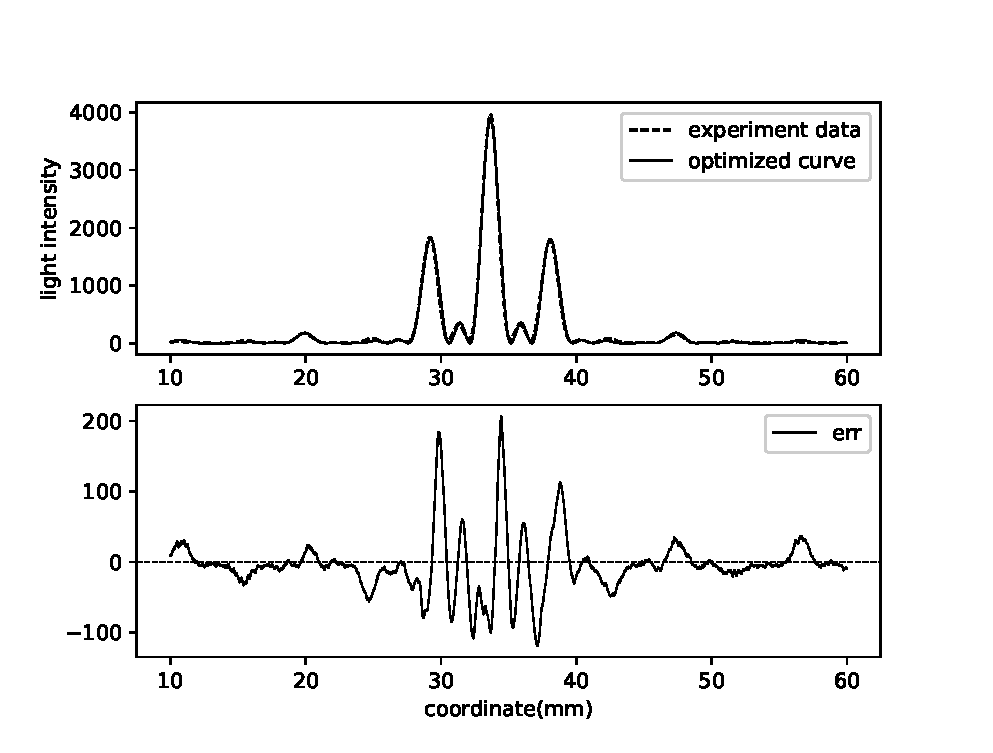
\includegraphics[scale=0.70]{image/triple_fit.eps}
        \caption{(1)拟合曲线与实验曲线的对比\;\;(2)残差图}
    \end{figure}
    \par 
    首先给出相关数据。探测器底座位置93.90cm,狭缝位置28.70cm,探测器与底座之间距离4mm,
    可以得到656mm。首先给出实验数据所绘制的衍射光强随探测器位置的分布。与双缝相比较
    可以看到,随着缝变多,光的能量开始向一些特定的点集中。
    \par 
    我们可以利用同样的公式(2)将里面的参数$N$改为3,继续使用相同的方法进行拟合,
    可以得到参数:$a = 42.8\;\mathrm{\mu m},\;\;d = 91.2\;\mathrm{\mu m}$。
    \par 
    从残差图上依然可以看出偏差有着与之前叙述相同的特点。
    \subsubsection{其他衍射屏的衍射图样}
    \begin{figure}[htbp]
        \centering
        \subfigure[单圆孔]{
        \includegraphics[width=4.5cm]{photo/circle.jpg}
        }
        \quad
        \subfigure[单方孔]{
        \includegraphics[width=4.5cm]{photo/single_square.jpg}
        }
    \quad
        \subfigure[单矩形孔]{
        \includegraphics[width=4.5cm]{photo/rectangular.jpg}
        }
    \quad
        \subfigure[等边三角形孔]{
        \includegraphics[width=4.5cm]{photo/triangle.jpg}
        }
    \quad
        \subfigure[五角星孔]{
        \includegraphics[width=4.5cm]{photo/star.jpg}
        }
    \quad
    \caption{单孔的衍射}
    \end{figure}

\par 
从上图可以看出,衍射图样与光屏形状有着明显的依赖关系,从某种程度上反映了衍射屏的
对称性,使得我们可以通过衍射图样来了解有关衍射屏的信息。
    \begin{figure}[htbp]
        \centering
        \quad
        \subfigure[双圆孔]{
        \includegraphics[width=5.5cm]{photo/double_circle.jpg}
        }
    \quad
    \quad
        \subfigure[双方孔]{
        \includegraphics[width=5.5cm]{photo/double_square.jpg}
        }
    \quad
    \caption{双孔的衍射}
    \end{figure}
    \par 
    双孔的衍射与单孔有着很明显的区别,出现了干涉条纹与更加精细的结构。
    \begin{figure}[htbp]
        \centering
        \subfigure[圆孔方阵]{
        \includegraphics[width=5.5cm]{photo/square_circle.jpg}
        }
    \quad
        \subfigure[方孔方阵]{
        \includegraphics[width=5.5cm]{photo/square_square.jpg}
        }
    \quad
    \caption{衍射单元排成方阵的衍射}
    \end{figure}
    \begin{figure}[htbp]
        \centering
        \subfigure[圆孔密排]{
        \includegraphics[width=5.5cm]{photo/closest_circle.jpg}
        }
    \quad
        \subfigure[方孔密排]{
        \includegraphics[width=5.5cm]{photo/closest_square.jpg}
        }
    \quad
    \caption{衍射单元密排的衍射}
    \end{figure}
    \par 
    从图 9,图 10 与之前的衍射图样对比可知,当衍射单元增加时,衍射条纹开始变得细锐
    与丰富;从图中很容易可以看出方阵与密排的区别,那么可以得出结论,衍射图样不仅反
    映衍射单元的对称性,同时反映了单元排布的对称性。方阵排布的衍射屏对应的衍射图样
    就具有4重对称性,而平面密排一定是按照平面密置单层的硬球那样,具有6重对称性,
    这同样也反映到了衍射图样中。
    \section{\large{分析与讨论}}
    \paragraph{夫琅禾费衍射图样与衍射屏结构之间的关系}
    考察由夫琅禾费衍射的定义装置导出的衍射场复振幅的表达式:
    $$
    \widetilde{U}(\theta_{1},\theta_{2}) = \widetilde{P} \cdot \iint \widetilde{t}(x,y) \cdot \mathrm{e}^{-\mathrm{i}k(\sin \theta_{1} x + \sin \theta_{2}y)}\mathrm{d}x\mathrm{d}y
    $$
    $$
    \widetilde{P} = \frac{-\mathrm{i}A_{1}}{\lambda r_{0}} \mathrm{e}^{\mathrm{i}r_{0}(\theta_{1},\theta_{2})}
    $$
    其中$\widetilde{t}(x, y)$是衍射屏的透射函数,是振幅与相位透射函数的乘积,若考虑屏的衍射,其应该
    是一个振幅型透射函数,透光部分取值为1,不透光部分取值为零。由于夫琅禾费衍射场的性质,衍射积分中只有
    一次的相位因子,从数学上看在不考虑积分前部分的$\widetilde{P}$(这是一个模为常数的因子)时,
    表达式相当于是对于屏函数$\widetilde{t}(x, y)$的傅里叶变换。如果要讨论光强,那么就相当于$|\widetilde{U}|^{2}$
    只需要用$|\widetilde{P}|^{2}$乘上屏函数傅里叶变换的模的平方即可。因此夫琅禾费衍射本质上是衍射屏
    函数的一个积分变换。
    \paragraph{有关曲线拟合的一点讨论}
    在拟合前面多缝衍射的光强分布曲线时,遇到了一些小问题,这引起了我对于使用软件拟合
    实验曲线的一些思考。前面拟合的函数,由于分母上可能为零,所以并不是每个点都有定义
    (每个点的函数值极限均存在,因此表达式本身有意义,但是拟合时是逐点计算,可能会出现
    分母为零的情况),因此严格按照实验数据拟合必然会出现程序报错的情况。考虑到这样的
    没有定义的点只有一个,光强最大值必然对应函数的奇异点,再考虑到探测器是以0.01mm为
    单位进行扫描,我们只需要在拟合时微小地改变一下参与拟合的数据,即把最大值的横坐标
    改动很小的值,这样就可以避免0的出现,同时对于整个曲线的形状几乎没有影响(试过
    在一定范围内改动值,对于图像和残差图均无可见的影响,还有这可不是篡改实验数据)。\\
    \\
    \section{\large{收获与感想}}
    \par 
    感想就是实验挺有意思的,实验报告费了我很大的功夫,收获就是实验报告在
    费了很大功夫的同时,我的数据处理能力有所提高。
\end{document}